%\documentclass[12pt,handout]{beamer}
\documentclass[presentation]{beamer}
\usepackage{../oop-slides-lab}

\setbeamertemplate{bibliography item}[text]

\newcommand{\lab}{Lab05}

\title[{\lab} -- DVCS2]{Distributed Version Control Systems II \\
Branching e merging}

\date[\today]{\today}

\begin{document}
	
\frame[label=coverpage]{\titlepage}

\newcommand{\al}[0]{\textless}
\newcommand{\ar}[0]{\textgreater}
\newcommand{\gen}[1]{\al{}#1\ar{}}
\newcommand{\imgfr}[4]{\fr{#1}{#2
\begin{center}
\includegraphics[width=#3\textwidth]{#4}                    
\end{center}
}}

\section{Navigazione della storia, branching, e merging}

\subsection{Concetti fondamentali}

\begin{frame}[allowframebreaks]{Concetti basilari e terminologia}
	\begin{block}{Navigazione della storia}
		Possibilità di tornare ad un qualunque commit (salvataggio) precedente o successivo
	\end{block}
	\begin{block}{Branch}
		Linea di sviluppo (ossia sequenza di commit successivi). Dal momento in cui si può tornare indietro nella storia dei salvataggi e ripartire a sviluppare, si può creare una nuova linea di sviluppo, che si diparte da quella originale e procede parallelamente.
		\begin{center}
			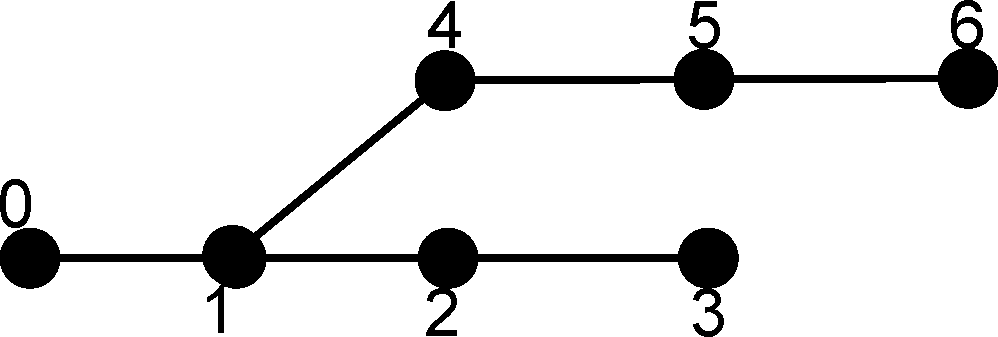
\includegraphics[height=.4\textheight]{img/branch}
		\end{center}
	\end{block}
	\begin{block}{Head}
		Identifica la posizione corrente all'interno della storia del repository.
		È in sostanza un riferimento ad uno specifico commit.
		In una normale sessione di lavoro, la \texttt{HEAD} è posizionata alla fine di un branch.
		Quando si naviga nella storia del repository, lo si fa spostando la \texttt{HEAD}.
	\end{block}
	\begin{block}{Merge}
		Fusione di due branch (linee di sviluppo) in una sola.
		\begin{center}
			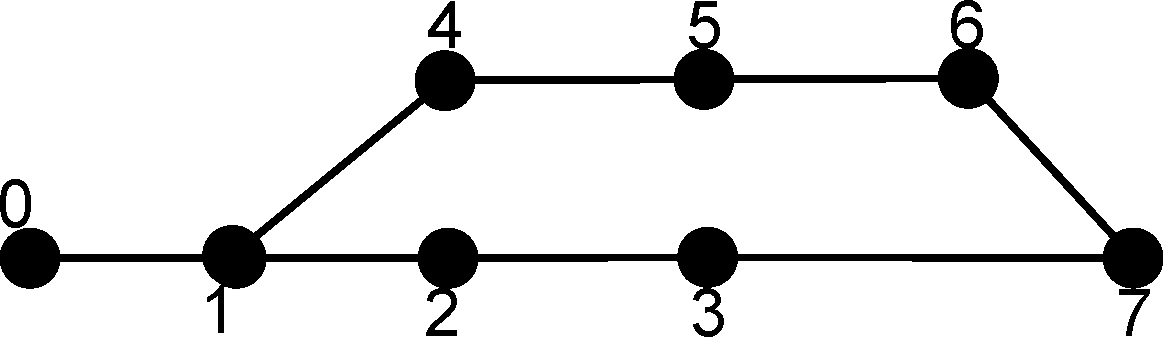
\includegraphics[width=.99\textwidth]{img/merge}
		\end{center}
	\end{block}
\end{frame}

\subsection{Visualizzazione della linea di sviluppo}

\begin{frame}[allowframebreaks,fragile]{Visualizzazione della storia}
	\begin{block}{In generale}
		Visualizzare l'elenco dei commit effettuati, chi li ha eseguiti, quando, ed il loro message commit
	\end{block}
	\begin{block}{In Git}
		Git offre il sottocomando \texttt{log}
		\begin{itemize}
			\item \texttt{git log}
			\begin{itemize}
				\item Visualizza tutti i commit della linea di sviluppo corrente
				\item Se l'output è troppo lungo crea una visualizzazione scorrevole (si vedano i comandi Unix \texttt{less} e \texttt{more})
				\item Per uscire dalla visualizzazione scorrevole, si usa il tasto Q
			\end{itemize}
			\item \texttt{git log --graph}
			\begin{itemize}
				\item Come sopra, con visualizzazione grafica dell'evoluzione sulla sinistra 
			\end{itemize}
		\end{itemize}
	\end{block}
	\begin{block}{Esercizio}
		\begin{itemize}
            \item Si riparta dal repository contenente l'esercizio eseguito nella lezione precedente
            \begin{itemize}
                \item Nel caso in cui non fosse stato completato, esso è reso disponibile assieme 
agli esercizi
            \end{itemize}
			\item Si visualizzi l'attuale storia del repository, corredata di grafico
		\end{itemize}
	\end{block}
	\begin{block}{Output atteso}
		\begin{Verbatim}[fontsize=\tiny]
* commit 47b5f2fb9f5300dc8bc530ce45d37a86a0436755
| Author: Danilo Pianini <danilo.pianini@unibo.it>
| Date:   Wed Oct 19 16:46:21 2016 +0200
| 
|     Remove the trash
|  
* commit 4d086a9b0d2139f0cd300d329f532a2c464304c7
| Author: Danilo Pianini <danilo.pianini@unibo.it>
| Date:   Wed Oct 19 16:45:28 2016 +0200
| 
|     move junk to trash
|  
* commit 844aebd840e6f3d2b034312e9fa37677f64b9a15
| Author: Danilo Pianini <danilo.pianini@unibo.it>
| Date:   Wed Oct 19 16:43:48 2016 +0200
| 
|     Add junk
|  
* commit 3ae84225f45afdfa02c268c6079e0f6c96695c1f
| Author: Danilo Pianini <danilo.pianini@unibo.it>
| Date:   Wed Oct 19 16:26:30 2016 +0200
| 
|     Create .gitignore
|  
* commit 19aa252373d1e44897233bf5b733cf82019cd5bf
  Author: Danilo Pianini <danilo.pianini@unibo.it>
  Date:   Wed Oct 19 15:51:10 2016 +0200
  
      Create HelloWorld
		\end{Verbatim}
	\end{block}
\end{frame}

\begin{frame}[allowframebreaks,fragile]{Visualizzazione delle differenze}
	\begin{block}{In generale}
		Vogliamo poter controllare quali modifiche sono state introdotte da un commit
	\end{block}
	\begin{block}{In Git}
		Git può mostrare le modifiche fra intercorse fra due commit col sottocomando \texttt{diff}
		\begin{itemize}
			\item \texttt{git diff}
			\begin{itemize}
				\item Mostra le differenze fra il working tree e l'ultimo commit, \textit{escludendo il contenuto della staging area}
			\end{itemize}
			\item \texttt{git diff FROM}
			\begin{itemize}
				\item Dove \texttt{FROM} è un riferimento ad un commit
				\item Mostra le differenze fra \texttt{FROM} e il working tree
			\end{itemize}
			\item \texttt{git diff FROM TO}
			\begin{itemize}
				\item Dove \texttt{FROM} e \texttt{TO} sono gli hash di due commit
				\item Mostra le differenze fra \texttt{FROM} e \texttt{TO}
			\end{itemize}
		\end{itemize}
		Il formato dell'output è lo stesso del comando Unix \texttt{diff}, è interpretabile da quest'ultimo e può essere utilizzato per creare delle ``patch''.
	\end{block}
	\begin{block}{\texttt{HEAD}}
		Per semplificare l'accesso agli ultimi commit effettuati, Git mette a disposizione la keyword \texttt{HEAD}
		\begin{itemize}
			\item \texttt{HEAD} fa riferimento all'ultimo commit effettuato
			\item \texttt{HEAD\textasciitilde{}1} fa riferimento al penultimo commit effettuato
			\item \texttt{HEAD\textasciitilde{}2} fa riferimento al terz'ultimo commit effettuato
			\item \texttt{HEAD\textasciitilde{}N} fa riferimento al N-esimo commit effettuato prima dell'ultimo
		\end{itemize}
		È possibile quindi, ad esempio, richiedere di visualizzare le modifiche introdotte negli ultimi tre commit prima dell'ultimo usando:
		\begin{itemize}
			\item \texttt{git diff HEAD\textasciitilde{}3 HEAD}
		\end{itemize}
	\end{block}
	\begin{block}{Esercizio}	
		\begin{itemize}
			\item Osservare le differenze fra la staging area e i tre commit precedenti (\texttt{HEAD\textasciitilde{}2})
		\end{itemize}
	\end{block}
	\begin{block}{Output atteso}
		\begin{Verbatim}[fontsize=\scriptsize]
diff --git a/junk.txt b/junk.txt
deleted file mode 100644
index de0a8c8..0000000
--- a/junk.txt
+++ /dev/null
@@ -1 +0,0 @@
-some trash
		\end{Verbatim}
	\end{block}
		\begin{block}{Spiegazione dell'output}
		\begin{itemize}
			\item È stato cancellato un file con permessi ottali \texttt{644}
			\item è stato spostato \texttt{junk.txt} dentro \texttt{/dev/null}
			\begin{itemize}
				\item Ossia cancellato
				\item \texttt{/dev/null} è uno speciale device file Unix (lo vedrete in Sistemi Operativi)
			\end{itemize}
			\item Una modifica ha rimosso una linea a partire dalla riga 0, colonna 0
			\item Il contenuto della riga rimossa è \texttt{some trash}
		\end{itemize}
	\end{block}
\end{frame}

\subsection{Navigazione della linea di sviluppo}

\begin{frame}[allowframebreaks,fragile]{Navigazione della linea di sviluppo}
	\begin{block}{In generale}
		Vogliamo poter ritornare a qualunque salvataggio della nostra linea di sviluppo
	\end{block}
	\begin{block}{In Git}
		Il sottocomando \texttt{checkout} consente di ripristinare una versione precedente di un file o dell'intero repository
		\begin{itemize}
			\item \texttt{git checkout COMMITREF}
			\begin{itemize}
				\item Dove \texttt{COMMITREF} è lo hash di un commit o un suo riferimento, ad esempio:
				\begin{itemize}
					\item \texttt{HEAD}
					\item \texttt{master}, o altro nome di branch
				\end{itemize}
				\item Se non ci sono modifiche che rischiano di essere perse, torna al salvataggio \texttt{COMMITREF}
			\end{itemize}
			\item \texttt{git checkout COMMITREF -- FILENAME}
			\begin{itemize}
				\item Ripristina il file \texttt{FILENAME} prendendolo dal commit \texttt{COMMITREF}
			\end{itemize}
		\end{itemize}
	\end{block}
	\begin{block}{La modalità detached HEAD}
		Quando si torna indietro nella storia, Git entra in modalità ``detached HEAD'': la ``testa'', ossia il commit a cui ci troviamo, è staccato dalla ``cima'' della linea di sviluppo.\\
		\centering
		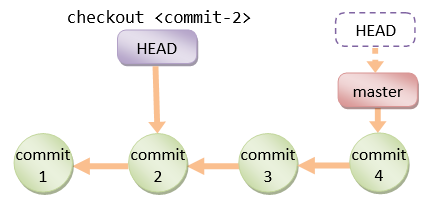
\includegraphics[width=.4\textwidth]{img/detached}
		\begin{itemize}
			\item I commit effettuati in questa modalità verranno scartati
			\item Per tornare alla modalità ``attached'', è necessario effettuare un checkout con il nome del branch
			\begin{itemize}
				\item Il nome del branch punta sempre all'ultimo commit su quella linea di sviluppo
				\item Ad esempio: \texttt{git checkout master}
			\end{itemize}
		\end{itemize}
	\end{block}
	\begin{block}{Esercizio}	
		Premessa: si osservi lo stato del repository con \texttt{git status} \textbf{prima e dopo ogni operazione}, assicurandosi di capire appieno l'output fornito da Git
		\begin{itemize}
			\item Si recuperi il file \texttt{junk.txt} da tre commit fa (\texttt{HEAD\textasciitilde{}2})
			\item Si vada al primo commit, usando il suo hash
			\begin{itemize}
				\item Potete ottenerlo usando \texttt{git log}
			\end{itemize}
			\item Si torni alla cima della linea di sviluppo (\texttt{master})
			\item Si rimuova il file \texttt{junk.txt} dall'area di staging (con \texttt{reset})
			\item Si elimini il file \texttt{junk.txt}
		\end{itemize}
	\end{block}
	\begin{block}{Output atteso}
		\begin{Verbatim}[fontsize=\scriptsize]
On branch master
nothing to commit, working tree clean
		\end{Verbatim}
	\end{block}
	\begin{block}{Output atteso}
		\begin{Verbatim}[fontsize=\scriptsize]
On branch master
Changes to be committed:
  (use "git reset HEAD <file>..." to unstage)

        new file:   junk.txt


		\end{Verbatim}
	\end{block}
	\begin{block}{Output atteso}
		\begin{Verbatim}[fontsize=\scriptsize]
A       junk.txt
Note: checking out '19aa252373d1e44897233bf5b733cf82019cd5bf'.

You are in 'detached HEAD' state. You can look around, make experimental
changes and commit them, and you can discard any commits you make in this
state without impacting any branches by performing another checkout.

If you want to create a new branch to retain commits you create, you may
do so (now or later) by using -b with the checkout command again. Example:

  git checkout -b <new-branch-name>

HEAD is now at 19aa252... Create HelloWorld
		\end{Verbatim}
	\end{block}
	\begin{block}{Output atteso}
		\begin{Verbatim}[fontsize=\scriptsize]
HEAD detached at 19aa252
Changes to be committed:
  (use "git reset HEAD <file>..." to unstage)

        new file:   junk.txt

Untracked files:
  (use "git add <file>..." to include in what will be committed)

        bin/

		\end{Verbatim}
	\end{block}
	\begin{block}{Output atteso}
		\begin{Verbatim}[fontsize=\scriptsize]
A       junk.txt
Previous HEAD position was 19aa252... Create HelloWorld
Switched to branch 'master
		\end{Verbatim}
	\end{block}
	\begin{block}{Output atteso}
		\begin{Verbatim}[fontsize=\scriptsize]
On branch master
Changes to be committed:
  (use "git reset HEAD <file>..." to unstage)

        new file:   junk.txt

		\end{Verbatim}
	\end{block}
	\begin{block}{Output atteso}
		\begin{Verbatim}[fontsize=\scriptsize]
On branch master
Untracked files:
  (use "git add <file>..." to include in what will be committed)

        junk.txt

nothing added to commit but untracked files present (use "git add" to track)
		\end{Verbatim}
	\end{block}
	\begin{block}{Output atteso}
		\begin{Verbatim}[fontsize=\scriptsize]
On branch master
nothing to commit, working tree clean
		\end{Verbatim}
	\end{block}
	\begin{block}{Spiegazione dell'output}
		\begin{itemize}
			\item Si noti che Git cerca di non cancellare le modifiche non salvate in un commit quando si naviga la storia (il file \texttt{junk.txt} non viene cancellato)
			\item In caso di conflitti, si rifiuterebbe di cambiare commit
			\item Si risolve cancellando le modifiche fatte o creando un nuovo commit, in modo da tornare allo stato di ``\texttt{working tree clean}''
		\end{itemize}
	\end{block}
\end{frame}

\subsection{Gestione di più linee di sviluppo}

\begin{frame}[allowframebreaks,fragile]{Creazione di nuove linee di sviluppo (branching)}
	\begin{block}{In generale}
		Vogliamo poter sviluppare su più linee
		\begin{itemize}
			\item Ad esempio perché stiamo per sviluppare una funzionalità che non sapremo se e quando completeremo, ma nel frattempo il nostro software va comunque manutenuto
			\item Ad esempio perché vogliamo sviluppare qualcosa a partire da una versione più vecchia (ossia, salvare i commit effettuati in modalità ``detached \texttt{HEAD}''
		\end{itemize}
	\end{block}
	\begin{block}{In Git}
		Il sottocomando \texttt{checkout} consente di creare passare di branch in branch, e di crearne di nuovi tramite l'opzione \texttt{-b}
		\begin{itemize}
			\item \texttt{git checkout -b branchname}
			\begin{itemize}
				\item Crea un nuovo branch di nome \texttt{branchname}
				\item I nuovi commit apparterranno a quel branch
			\end{itemize}
			\item \texttt{git checkout branchname}
			\begin{itemize}
				\item Passa dal branch corrente al branch \texttt{branchname}
				\item Questo in realtà è un ripasso di quanto detto un attimo fa...
			\end{itemize}
		\end{itemize}
		Il sottocomando \texttt{branch} consente di visualizzare i branch
		\begin{itemize}
			\item \texttt{git branch}
			\begin{itemize}
				\item Stampa i branch, mostrando con \texttt{*} quello corrente.
			\end{itemize}
		\end{itemize}
		L'opzione \texttt{--all} di \texttt{git log} visualizza la storia per tutti i branch
		\begin{itemize}
			\item \texttt{git log --all --graph}
		\end{itemize}
	\end{block}
	\begin{block}{Esercizio}	
		\textbf{Premessa}: si osservi e comprenda lo stato del repository con \texttt{git status} \textbf{prima e dopo ogni operazione} di modifica di file o \texttt{commit}
		\begin{itemize}
			\footnotesize
			\item Si visualizzino i branch disponibili
			\item Si crei un nuovo branch di nome \texttt{feature-readme}
			\item Si visualizzino i branch disponibili
			\item Si crei un nuovo file \texttt{README.md}, con del testo semplice
			\item Si aggiunga \texttt{README.md} alla staging area
			\item Si effettui il commit
			\item Si passi al branch \texttt{master}
			\item Si modifichi la stampa di \texttt{HelloWorld.java}
			\item Si aggiunga \texttt{HelloWorld.java} alla staging area
			\item Si effettui il commit
			\item Si visualizzi la storia dei commit su tutti i branch
		\end{itemize}
	\end{block}
	\begin{block}{Output atteso}
		\begin{Verbatim}[fontsize=\scriptsize]
* master
		\end{Verbatim}
	\end{block}
	\begin{block}{Output atteso}
		\begin{Verbatim}[fontsize=\scriptsize]
Switched to a new branch 'feature-readme'
		\end{Verbatim}
	\end{block}
	\begin{block}{Output atteso}
		\begin{Verbatim}[fontsize=\scriptsize]
* feature-readme
  master
		\end{Verbatim}
	\end{block}
	\begin{block}{Output atteso}
		\begin{Verbatim}[fontsize=\scriptsize]
On branch feature-readme
nothing to commit, working tree clean
		\end{Verbatim}
	\end{block}
	\begin{block}{Output atteso}
		\begin{Verbatim}[fontsize=\scriptsize]
On branch feature-readme
Untracked files:
  (use "git add <file>..." to include in what will be committed)

        README.md

nothing added to commit but untracked files present (use "git add" to track)
		\end{Verbatim}
	\end{block}
	\begin{block}{Output atteso}
		\begin{Verbatim}[fontsize=\scriptsize]
On branch feature-readme
Changes to be committed:
  (use "git reset HEAD <file>..." to unstage)

        new file:   README.md

		\end{Verbatim}
	\end{block}
	\begin{block}{Output atteso}
		\begin{Verbatim}[fontsize=\scriptsize]
[feature-readme 9261ec2] Add README.md file
 1 file changed, 1 insertion(+)
 create mode 100644 README.md
		\end{Verbatim}
	\end{block}
	\begin{block}{Output atteso}
		\begin{Verbatim}[fontsize=\scriptsize]
On branch feature-readme
nothing to commit, working tree clean
		\end{Verbatim}
	\end{block}
	\begin{block}{Output atteso}
		\begin{Verbatim}[fontsize=\scriptsize]
Switched to branch 'master'
		\end{Verbatim}
	\end{block}
	\begin{block}{Output atteso}
		\begin{Verbatim}[fontsize=\scriptsize]
On branch master
nothing to commit, working tree clean
		\end{Verbatim}
	\end{block}
	\begin{block}{Output atteso}
		\begin{Verbatim}[fontsize=\scriptsize]
On branch master
Changes not staged for commit:
  (use "git add <file>..." to update what will be committed)
  (use "git checkout -- <file>..." to discard changes in working directory)

        modified:   src/HelloWorld.java

no changes added to commit (use "git add" and/or "git commit -a")
		\end{Verbatim}
	\end{block}
	\begin{block}{Output atteso}
		\begin{Verbatim}[fontsize=\scriptsize]
On branch master
Changes to be committed:
  (use "git reset HEAD <file>..." to unstage)

        modified:   src/HelloWorld.java

		\end{Verbatim}
	\end{block}
	\begin{block}{Output atteso}
		\begin{Verbatim}[fontsize=\scriptsize]
[master 56aa7aa] Modify HelloWorld
 1 file changed, 1 insertion(+), 1 deletion(-)
		\end{Verbatim}
	\end{block}
	\begin{block}{Output atteso}
		\begin{Verbatim}[fontsize=\scriptsize]
On branch master
nothing to commit, working tree clean
		\end{Verbatim}
	\end{block}
	\begin{block}{Output atteso}
		\begin{Verbatim}[fontsize=\tiny]
* commit 56aa7aaad47026911c2aa2b026f33293c3b4fe31
| Author: Danilo Pianini <danilo.pianini@unibo.it>
| Date:   Thu Oct 20 15:47:57 2016 +0200
| 
|     Modify HelloWorld
|    
| * commit 9261ec24cfb56d7cd7ecc67d4eaa8add9c44b3ff
|/  Author: Danilo Pianini <danilo.pianini@unibo.it>
|   Date:   Thu Oct 20 15:43:50 2016 +0200
|   
|       Add README.md file
|  
* commit 47b5f2fb9f5300dc8bc530ce45d37a86a0436755
| Author: Danilo Pianini <danilo.pianini@unibo.it>
| Date:   Wed Oct 19 16:46:21 2016 +0200
| 
|     Remove the trash
|  
* commit 4d086a9b0d2139f0cd300d329f532a2c464304c7
| Author: Danilo Pianini <danilo.pianini@unibo.it>
| Date:   Wed Oct 19 16:45:28 2016 +0200
| 
|     move junk to trash

... CONTINUA!
		\end{Verbatim}
	\end{block}
\end{frame}

\begin{frame}[allowframebreaks,fragile]{Unione di più linee di sviluppo (merge)}
	\begin{block}{In generale}
		Vogliamo poter unire due linee di sviluppo in una sola
		\begin{itemize}
			\item Abbiamo sviluppato in un branch separato una nuova funzionalità, ora è pronta e vogliamo unirla al resto
		\end{itemize}
	\end{block}
	\begin{block}{In Git}
		Il sottocomando \texttt{merge} consente di unire due branch
		\begin{itemize}
			\item \texttt{git merge branchname}
			\begin{itemize}
				\item Tenta di unire le modifiche di \texttt{branchname} al branch corrente
				\item Prima di effettuare il merge, è necessario spostarsi sul branch destinazione (con \texttt{checkout})
				\item Se non ci sono conflitti, tutti i commit di \texttt{branchname} vengono aggiunti al branch corrente
				\item Viene creato un nuovo commit (merge commit)
				\item È buona norma non cambiare il messaggio di commit predefinito
				\item La risoluzione dei conflitti sarà uno dei temi del prossimo laboratorio
			\end{itemize}
			\item \texttt{git branch -d branchname}
			\begin{itemize}
				\item Elimina il branch \texttt{branchname}
				\item Se un branch non dovesse più servire, ad esempio perché tutte le sue modifiche sono state merse in un altro branch, è possibile rimuoverlo.
			\end{itemize}
		\end{itemize}
	\end{block}
	\begin{block}{Esercizio}	
		\textbf{Premessa}: si osservi e comprenda lo stato del repository con \texttt{git status} \textbf{prima e dopo ogni operazione} di modifica di file o \texttt{merge}
		\begin{itemize}
			\footnotesize
			\item Si visualizzino i branch disponibili, ci si assicuri di essere su \texttt{master}
			\item Si faccia il merge di \texttt{feature-readme}
			\item Si visualizzino i file del repository con \texttt{ls -ahl} (Unix) o \texttt{dir} (Windows)
			\item Si visualizzi la storia dei commit su tutti i branch
			\item Si elimini il branch \texttt{feature-readme}
			\item Si visualizzino i branch disponibili
			\item Si visualizzi la storia dei commit su tutti i branch
		\end{itemize}
	\end{block}
	\begin{block}{Output atteso}
		\begin{Verbatim}[fontsize=\scriptsize]
  feature-readme
* master
		\end{Verbatim}
	\end{block}
	\begin{block}{Output atteso}
		\begin{Verbatim}[fontsize=\scriptsize]
On branch master
nothing to commit, working tree clean
		\end{Verbatim}
	\end{block}
	\begin{block}{Output atteso}
		\begin{Verbatim}[fontsize=\scriptsize]
Merge made by the 'recursive' strategy.
 README.md | 1 +
 1 file changed, 1 insertion(+)
 create mode 100644 README.md
		\end{Verbatim}
	\end{block}
	\begin{block}{Output atteso}
		\begin{Verbatim}[fontsize=\scriptsize]
On branch master
nothing to commit, working tree clean
		\end{Verbatim}
	\end{block}
	\begin{block}{Output atteso}
		\begin{Verbatim}[fontsize=\scriptsize]
total 2.0M
drwxr-xr-x 5 danysk users 4.0K Oct 20 16:15 .
drwxr-xr-x 6 danysk users 2.0M Oct 20 15:56 ..
drwxr-xr-x 2 danysk users 4.0K Oct 19 16:22 bin
drwxr-xr-x 8 danysk users 4.0K Oct 20 16:15 .git
-rw-r--r-- 1 danysk users    5 Oct 19 18:55 .gitignore
-rw-r--r-- 1 danysk users   25 Oct 20 16:15 README.md
drwxr-xr-x 2 danysk users 4.0K Oct 19 16:00 src
		\end{Verbatim}
	\end{block}
	\begin{block}{Output atteso}
		\begin{Verbatim}[fontsize=\tiny]
*   commit b68c8a48dc24bd1d948c2ac4409d8d91a000b8b6
|\  Merge: 56aa7aa 9261ec2
| | Author: Danilo Pianini <danilo.pianini@unibo.it>
| | Date:   Thu Oct 20 16:15:47 2016 +0200
| | 
| |     Merge branch 'feature-readme'
| |   
| * commit 9261ec24cfb56d7cd7ecc67d4eaa8add9c44b3ff
| | Author: Danilo Pianini <danilo.pianini@unibo.it>
| | Date:   Thu Oct 20 15:43:50 2016 +0200
| | 
| |     Add README.md file
| |   
* | commit 56aa7aaad47026911c2aa2b026f33293c3b4fe31
|/  Author: Danilo Pianini <danilo.pianini@unibo.it>
|   Date:   Thu Oct 20 15:47:57 2016 +0200
|   
|       Modify HelloWorld
|  
* commit 47b5f2fb9f5300dc8bc530ce45d37a86a0436755
| Author: Danilo Pianini <danilo.pianini@unibo.it>
| Date:   Wed Oct 19 16:46:21 2016 +0200
| 
|     Remove the trash
|  

...CONTINUA!
		\end{Verbatim}
	\end{block}
	\begin{block}{Output atteso}
		\begin{Verbatim}[fontsize=\scriptsize]
Deleted branch feature-readme (was 9261ec2).
		\end{Verbatim}
	\end{block}
	\begin{block}{Output atteso}
		\begin{Verbatim}[fontsize=\scriptsize]
* master
		\end{Verbatim}
	\end{block}
	\begin{block}{Output atteso}
		\begin{Verbatim}[fontsize=\tiny]
*   commit b68c8a48dc24bd1d948c2ac4409d8d91a000b8b6
|\  Merge: 56aa7aa 9261ec2
| | Author: Danilo Pianini <danilo.pianini@unibo.it>
| | Date:   Thu Oct 20 16:15:47 2016 +0200
| | 
| |     Merge branch 'feature-readme'
| |   
| * commit 9261ec24cfb56d7cd7ecc67d4eaa8add9c44b3ff
| | Author: Danilo Pianini <danilo.pianini@unibo.it>
| | Date:   Thu Oct 20 15:43:50 2016 +0200
| | 
| |     Add README.md file
| |   
* | commit 56aa7aaad47026911c2aa2b026f33293c3b4fe31
|/  Author: Danilo Pianini <danilo.pianini@unibo.it>
|   Date:   Thu Oct 20 15:47:57 2016 +0200
|   
|       Modify HelloWorld
|  
* commit 47b5f2fb9f5300dc8bc530ce45d37a86a0436755
| Author: Danilo Pianini <danilo.pianini@unibo.it>
| Date:   Wed Oct 19 16:46:21 2016 +0200
| 
|     Remove the trash
|  

...CONTINUA!
		\end{Verbatim}
	\end{block}
\end{frame}

\begin{frame}{Conclusioni}
	\begin{itemize}
		\item Avete in mano uno strumento molto potente
		\item Usatelo sempre d'ora in poi
		\item A partire da questo laboratorio!
		\begin{itemize}
			\item Effettuate almeno un commit alla fine di ogni esercizio prima di chiamarci per correggere
			\item Se ve ne servono di più, fatene di più!
		\end{itemize}
	\end{itemize}
	\begin{block}{Nei prossimi laboratori}
		\begin{itemize}
			\item Impareremo ad usare git per lavorare in modo efficace con un team di persone
			\item Impareremo a scambiarci commit via Internet
			\item Lo useremo per ottenere le esercitazioni (bye bye zip files)
		\end{itemize}
	\end{block}
	\begin{block}{Nel progetto d'esame}
		\begin{itemize}
			\item Andrà consegnato sotto forma di repository Git o Mercurial
			\item L'abilità nell'uso del DVCS sarà parte della valutazione
		\end{itemize}
	\end{block}
\end{frame}

\end{document}
